\documentclass[12pt,a4paper,final]{article}
\usepackage[left=2.5cm,right=2.5cm,top=2.5cm,bottom=2.5cm]{geometry}

%% IDIOMA
\usepackage[utf8]{inputenc}
\usepackage[portuguese]{babel}

%% TRANSFORMAÇÕES ESTILO CSS
\usepackage{graphicx}

%% ESTÉTICA
\usepackage{enumerate}
\usepackage{booktabs}
\usepackage{amsmath, amsthm, amssymb, amsfonts}
\usepackage{multirow}
\usepackage[hyphens]{url}
\usepackage{subfig}

%% FONTE
\usepackage[T1]{fontenc}
%\usepackage[sc]{mathpazo} % Palatino with smallcaps
\usepackage{mathptmx}
\usepackage{eulervm} % Euler math

%% TIPOGRAFIA
\usepackage{parskip}
\usepackage[activate={true,nocompatibility},final,tracking=true,kerning=true,spacing=true,factor=1100,stretch=10,shrink=10]{microtype}

%% CODIGO
\usepackage{listings}
\usepackage{color}

\definecolor{dkgreen}{rgb}{0,0.6,0}
\definecolor{gray}{rgb}{0.5,0.5,0.5}
\definecolor{mauve}{rgb}{0.58,0,0.82}

\lstset{frame=tb,
  aboveskip=3mm,
  belowskip=3mm,
  showstringspaces=false,
  columns=flexible,
  basicstyle={\small\ttfamily},
  numbers=none,
  numberstyle=\tiny\color{gray},
  keywordstyle=\color{blue},
  commentstyle=\color{dkgreen},
  stringstyle=\color{mauve},
  breaklines=true,
  breakatwhitespace=true,
  tabsize=3
}

\title{Relatório 11 de TCC2/IC}
\author{Ly Sandro Amorim de Campos Salles\\Departamento de Física\\Universidade Federal do Paraná}
\date{\today}

\begin{document}
	\maketitle

  Desde o último encontro foram realizadas as seguintes atividades:

  Considerando que computadores geram números aleatórios a partir de uma \textit{seed}, foi verificada a presença de caos nas simulações com vizinhança de Moore utilizando o seguinte método:
  \begin{enumerate}
    \item Geração da matriz inicial com a \textit{seed} $156501936$ (gerada em uma calculadora Casio);
    \item Inversão de estado e limiar de $n$ células em posições aleatórias geradas com \textit{seed} baseada no horário mundial;
    \item Execução da simulação para 10000 ciclos utilizando $L=100$, limiar igual a $q$ e \textit{seed} igual a $2376222$ (gerada em uma Casio);
  \end{enumerate}
  Esse procedimento foi feito para $n\in\{0, 1, 10, 100, 1000, 10000\}$ e $q\in\{0.1, 1, 2, 3, 4, 5, 6, 7, 8, 9, 10\}$.

  A verificação da existência de caos foi feita considerando o coeficiente de Lyapunov
  \begin{align}
    \lambda = \dfrac{1}{n} \mathrm{ln}\left|\dfrac{f^n(x+\varepsilon) - f^n(x_0)}{\varepsilon}\right| = \dfrac{1}{n} \mathrm{ln}(\Delta)
  \end{align}
  Porém, considerando que $\mathrm{ln}(0)=-\infty$ e que computadores não lidam muito bem com infinito, foram feitas as seguintes observações com o intuito de desenvolver um coeficiente equivalente:
  \begin{enumerate}[a)]
    \item $\forall \Delta > 0$ tem-se que $\lambda < 0 \Leftrightarrow \mathrm{e}^\lambda < 1 \Leftrightarrow \Delta^\frac{1}{n} < 1 \Leftrightarrow \Delta^\frac{1}{10} < 1 \Rightarrow$ sistema estável 
    \item $\forall \Delta > 0$ tem-se que $\lambda = 0 \Leftrightarrow \mathrm{e}^\lambda = 1 \Leftrightarrow \Delta^\frac{1}{n} = 1 \Leftrightarrow \Delta^\frac{1}{10} = 1$ 
    \item $\forall \Delta > 0$ tem-se que $\lambda > 0 \Leftrightarrow \mathrm{e}^\lambda > 1 \Leftrightarrow \Delta^\frac{1}{n} > 1 \Leftrightarrow \Delta^\frac{1}{10} > 1 \Rightarrow$ sistema caótico 
  \end{enumerate}
 (O número 10 foi tomado arbitrariamente com a finalidade de diminuir números grandes). Portanto, é suficiente mostrar que $\Delta^\frac{1}{10} > 1$. A tabela \ref{tab:mediaDelta} lista os valores médios de $\Delta^\frac{1}{10}$ para matrizes iniciais que tiveram até $10^x\%$ de suas células modificadas, com $x\in\{-2, -1, 0, 1, 2\}$.

 \begin{table}[h]
  \centering
  \begin{tabular}{c ccccc}
    \toprule
    q & \multicolumn{5}{c}{Valor médio de $\Delta^\frac{1}{10}$ para $\varepsilon$ máximo de}\\
     & 0.01\% & 0.1\% & 1\% & 10\% & 100\%\\\midrule
    0.1 & 1.8794	& 1.8456	& 1.7018	& 1.4393	& 1.8960\\
    1.0 & 1.8958	& 1.7182	& 1.5883	& 1.4302	& 1.2938\\
    2.0 & 2.0125	& 2.3890	& 1.6698	& 1.6073	& 1.5662\\
    3.0 & 1.2384	& 1.7053	& 1.9184	& 1.4607	& 1.4430\\
    4.0 & 1.3701	& 2.4282	& 1.9308	& 1.7997	& 1.3555\\
    5.0 & 1.8896	& 1.6471	& 1.5051	& 2.2331	& 1.2264\\
    6.0 & 1.5401	& 1.3400	& 1.4389	& 1.0733	& 1.1573\\
    7.0 & 1.5848	& 1.4721	& 1.3281	& 1.1638	& 1.1869\\
    8.0 & 1.3449	& 1.3471	& 1.2113	& 1.2330	& 1.0450\\
    9.0 & 1.4383	& 1.4295	& 1.2436	& 1.0116	& 1.0921\\
    10.0& 1.3170	& 1.7878	& 1.2356	& 1.2074	& 1.2092\\\bottomrule
  \end{tabular}
  \caption{Valores médios para $\Delta^\frac{1}{10}$ obtidos na simulação com Vizinhança de Moore. Apesar de todos serem positivos, indicando a presença de cáos, alguns são próximos de $1$, indicando sistemas menos caóticos no intervalo de ciclos observado.}
  \label{tab:mediaDelta}
  \end{table}

  \begin{figure}
    \centering
    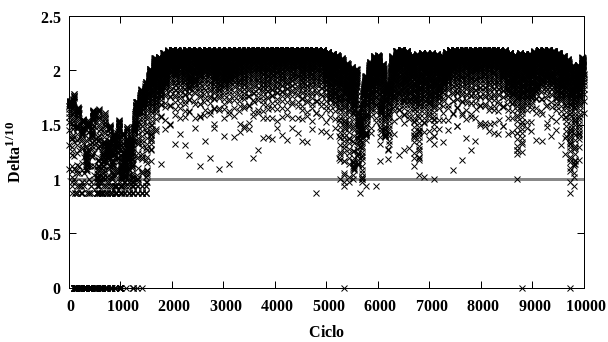
\includegraphics[width=0.7\textwidth]{caosq01noise10.png}
    \caption{$\Delta^\frac{1}{10}$ ao longo de 10000 ciclos de uma simulação com $L=100$, $q=0.1$, vizinhança de Moore, e $\varepsilon$ de até $0.1\%$ de diferença com a matriz inicial. O sistema tende a se comportar de forma parecida com o original durante os primeiros 1500 ciclos, tendo um ponto crítico a partir do ciclo 1500, a partir do qual o sistema fica totalmente caótico.}
    \label{fig:caosq01noise10}
  \end{figure}

  Para os próximos dias, estas serão as tarefas realizadas:
  \begin{enumerate}
    \item Verificação de comportamento caótico para o autômato celular considerando a vizinhança Von Neumann;
    \item Demonstração matemática do Algoritmo de Contagem de Aglomerados utilizado;
    \item Desenvolvimento da explicação que considera $q$ como liquidez;
    \item Desenvolvimento da explicação que considera $q$ como volatilidade;
    \item Explicação do porquê de o limiar intrínseco a cada célula ser considerado como um determinador do momento certo para vender ou comprar, no caso de $q$ ser considerado como liquidez;
    \item Leitura de Referênciais Teóricos apropriados para os trabalhos desenvolvidos;
    \item Escrita do TCC.
	\end{enumerate}

\end{document}
